\subsection{Diagramas de Componentes de package Pantallas}

Para una comprensión más profunda de la arquitectura de la interfaz de usuario de la aplicación móvil, a continuación se presentan los diagramas de componentes para cada una de las pantallas principales. Estos diagramas ilustran la composición interna de cada pantalla, mostrando los elementos de la interfaz de usuario (Composables), los datos que manejan y las posibles interacciones o dependencias con otros componentes. Cada diagrama proporciona una vista modular de la pantalla, facilitando la visualización de cómo se construyen las distintas secciones de la interfaz de usuario y cómo se relacionan entre sí. La Figura \ref{fig:Pantallas} muestra las pantallas (archivos .kt) presentes en package.Pantallas.

\begin{figure}[htbp!]
	\begin{center}
		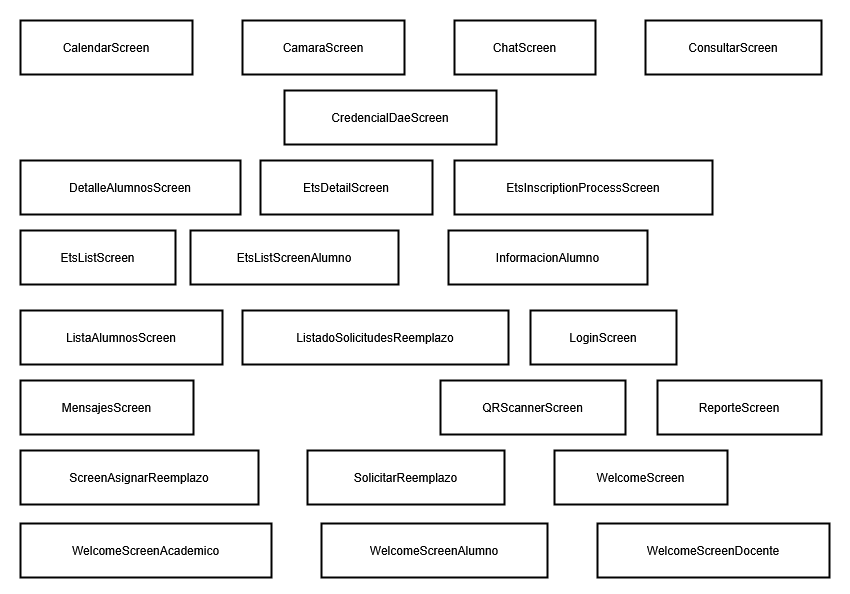
\includegraphics[width=0.9\textwidth]{DiagramasMoviles/DCM (12)}
		\caption{Pantallas presentes en package.Pantallas (archivos .kt).}
		\label{fig:Pantallas}
	\end{center}
\end{figure}


\newpage

\subsection{Diagrama de Componentes de CalendarScreen.kt}

La Figura \ref{fig:Componentes_1} muestra el diagrama de componentes para CalendarScreen.kt que es un composable que contiene a la \IUref{IU02}{Pantalla Consultar calendario escolar}, que muestra el calendario escolar y permite al usuario ver cuantos días faltan para el periodo de ETS próximo si esta disponible.

\begin{figure}[htbp!]
	\begin{center}
		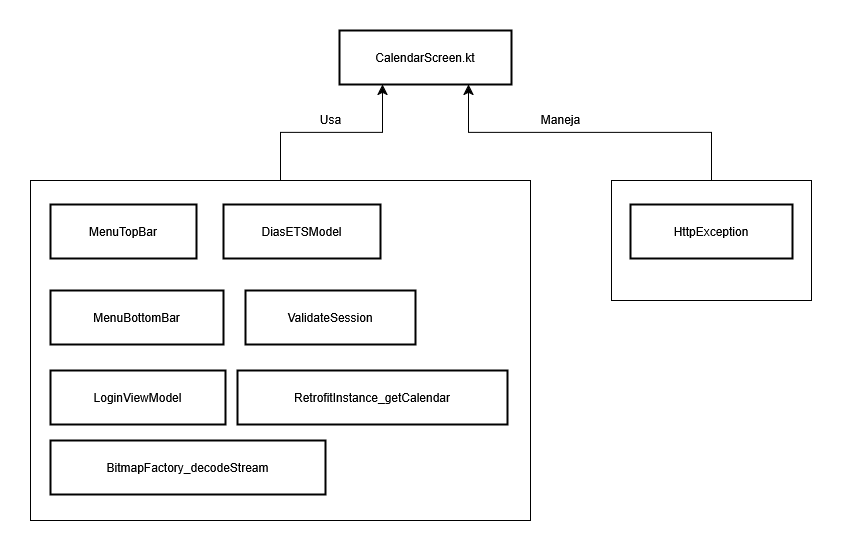
\includegraphics[width=0.9\textwidth]{DiagramasMoviles/DCM (13)}
		\caption{Diagrama de componentes para CalendarScreen.kt .}
		\label{fig:Componentes_1}
	\end{center}
\end{figure}

\newpage

\subsection{Diagrama de Componentes de CamaraScreen.kt}

La Figura \ref{fig:Componentes_2} muestra el diagrama de componentes para CamaraScreen.kt que es un composable que contiene a la \IUref{IU17}{Pantalla de Reconocimiento facial} y la \IUref{IU19}{Pantalla de Reconocimiento facial alumno}, que muestran la cámara usada para obtener la foto que se usara para el proceso de reconocimiento facial.

\begin{figure}[htbp!]
	\begin{center}
		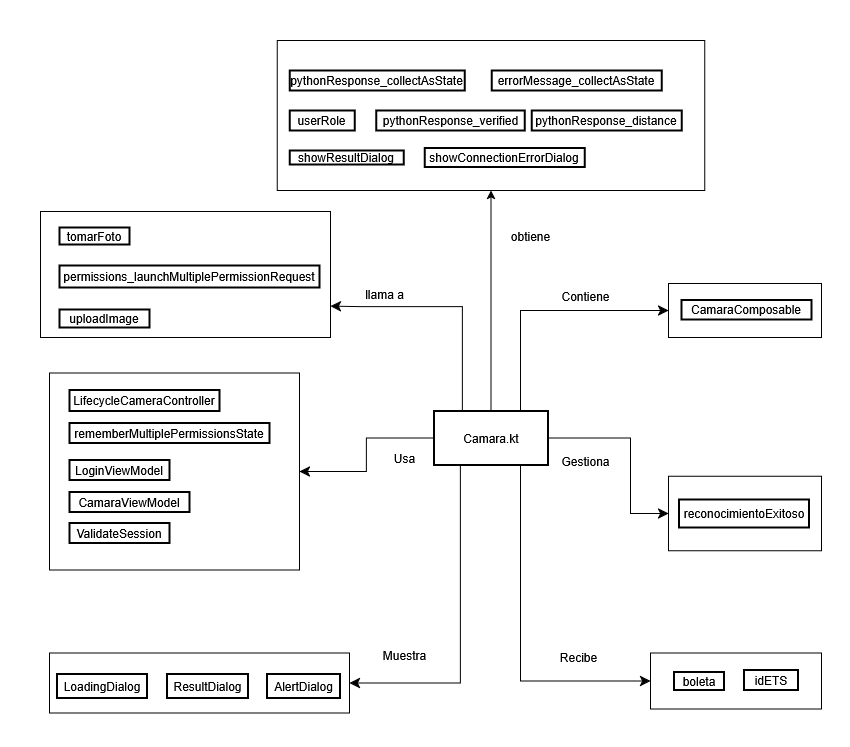
\includegraphics[width=0.9\textwidth]{DiagramasMoviles/DCM (14)}
		\caption{Diagrama de componentes para CamaraScreen.kt .}
		\label{fig:Componentes_2}
	\end{center}
\end{figure}

\newpage

\subsection{Diagrama de Componentes de ChatScreen.kt}

La Figura \ref{fig:Componentes_3} muestra el diagrama de componentes para ChatScreen.kt que es un composable que contiene una pantalla que muestra el chat de mensajes que pueden usar los usuarios.

\begin{figure}[htbp!]
	\begin{center}
		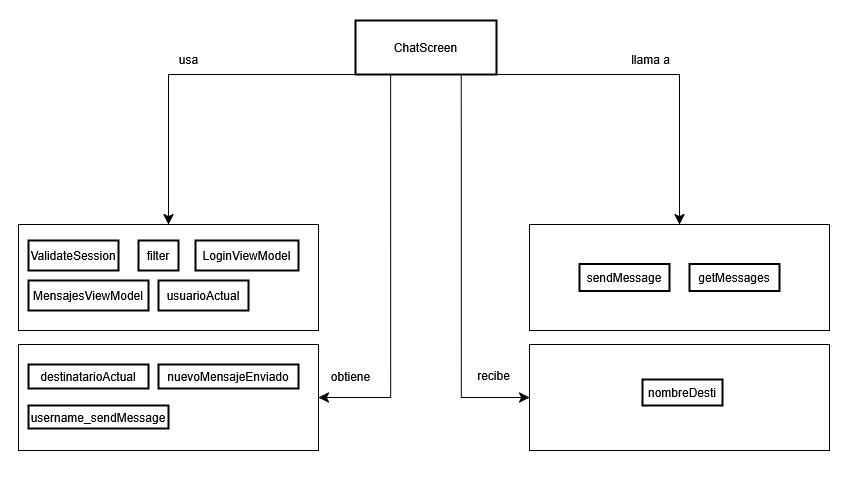
\includegraphics[width=0.9\textwidth]{DiagramasMoviles/DCM (15)}
		\caption{Diagrama de componentes para ChatScreen.kt .}
		\label{fig:Componentes_3}
	\end{center}
\end{figure}

\newpage

\subsection{Diagrama de Componentes de ConsultarScreen.kt}

La Figura \ref{fig:Componentes_4} muestra el diagrama de componentes para ConsultarScreen.kt que es un composable que contiene a la \IUref{IU12}{Pantalla Buscar alumno}, que muestra la lista de los alumnos inscritos a un ETS para el personal de seguridad y le permite filtrarlos por nombre o boleta.

\begin{figure}[htbp!]
	\begin{center}
		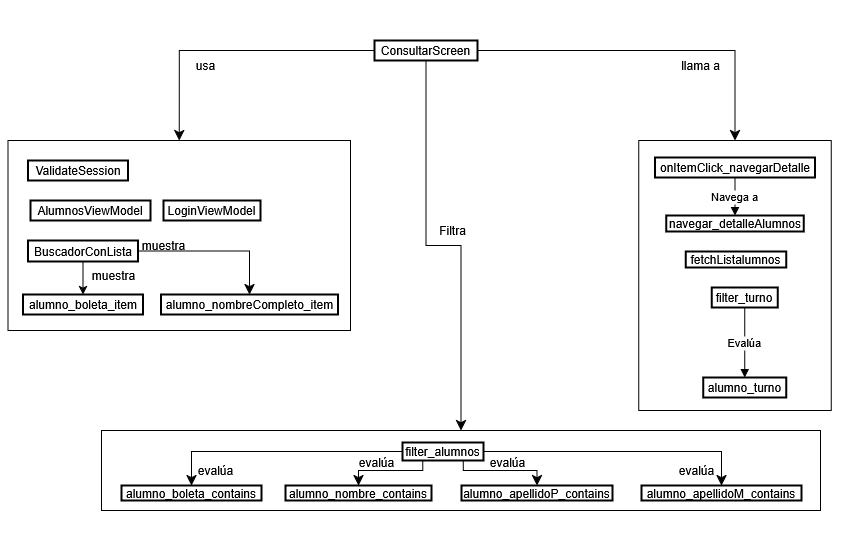
\includegraphics[width=0.9\textwidth]{DiagramasMoviles/DCM (16)}
		\caption{Diagrama de componentes para ConsultarScreen.kt .}
		\label{fig:Componentes_4}
	\end{center}
\end{figure}

\newpage

\subsection{Diagrama de Componentes de CredencialDaeScreen.kt}

La Figura \ref{fig:Componentes_5} muestra el diagrama de componentes para CredencialDaeScreen.kt que es un composable que contiene a la \IUref{IU11}{Pantalla Credencial del alumno}, que muestra la comparación de la credencial de la DAE con la credencial creada por el sistema.

\begin{figure}[htbp!]
	\begin{center}
		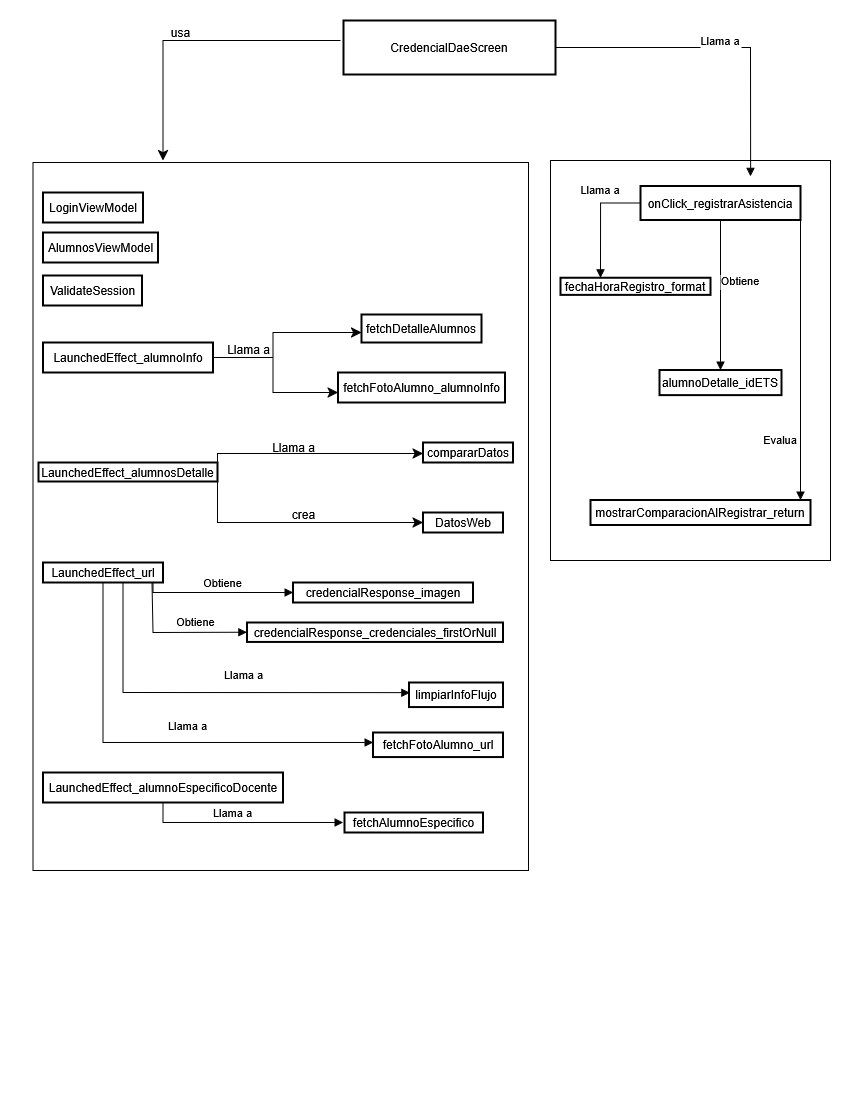
\includegraphics[width=0.9\textwidth]{DiagramasMoviles/DCM (17)}
		\caption{Diagrama de componentes para CredencialDaeScreen.kt .}
		\label{fig:Componentes_5}
	\end{center}
\end{figure}

\newpage

\subsection{Diagrama de Componentes de DetallesAlumnosScreen.kt}

La Figura \ref{fig:Componentes_6} muestra el diagrama de componentes para DetallesAlumnosScreen.kt que es un composable que contiene a la \IUref{IU11}{Pantalla Credencial del alumno}, que en este caso muestra la información relevante del alumno.

\begin{figure}[htbp!]
	\begin{center}
		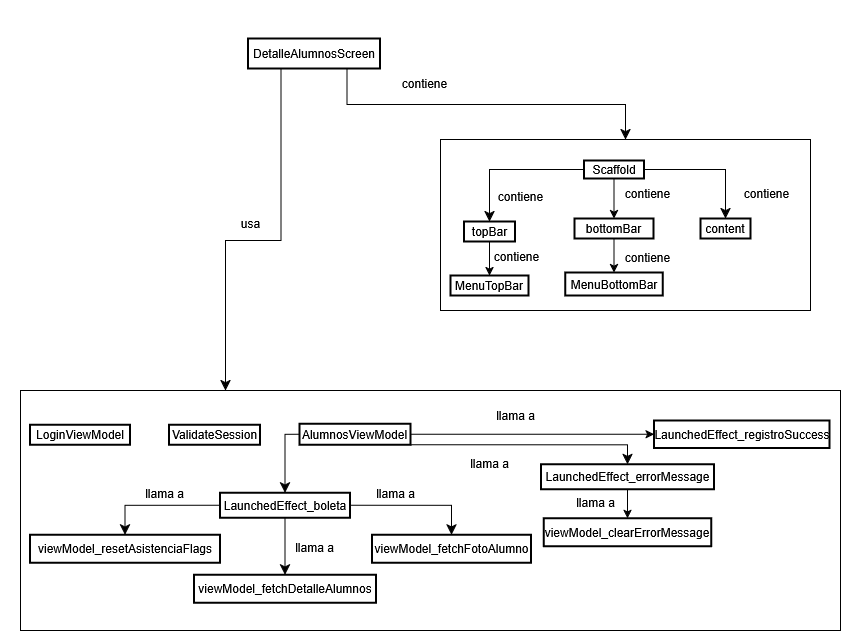
\includegraphics[width=0.9\textwidth]{DiagramasMoviles/DCM (19)}
		\caption{Diagrama de componentes para DetallesAlumnosScreen.kt .}
		\label{fig:Componentes_6}
	\end{center}
\end{figure}

\newpage

\subsection{Diagrama de Componentes de EtsDetailScreen.kt}

La Figura \ref{fig:Componentes_7} muestra el diagrama de componentes para EtsDetailScreen.kt que es un composable que contiene a la \IUref{IU06}{Pantalla Información de ETS} y \IUref{IU16}{Pantalla Información de ETS del alumno}, que muestra la información del ETS elegido por el usuario.

\begin{figure}[htbp!]
	\begin{center}
		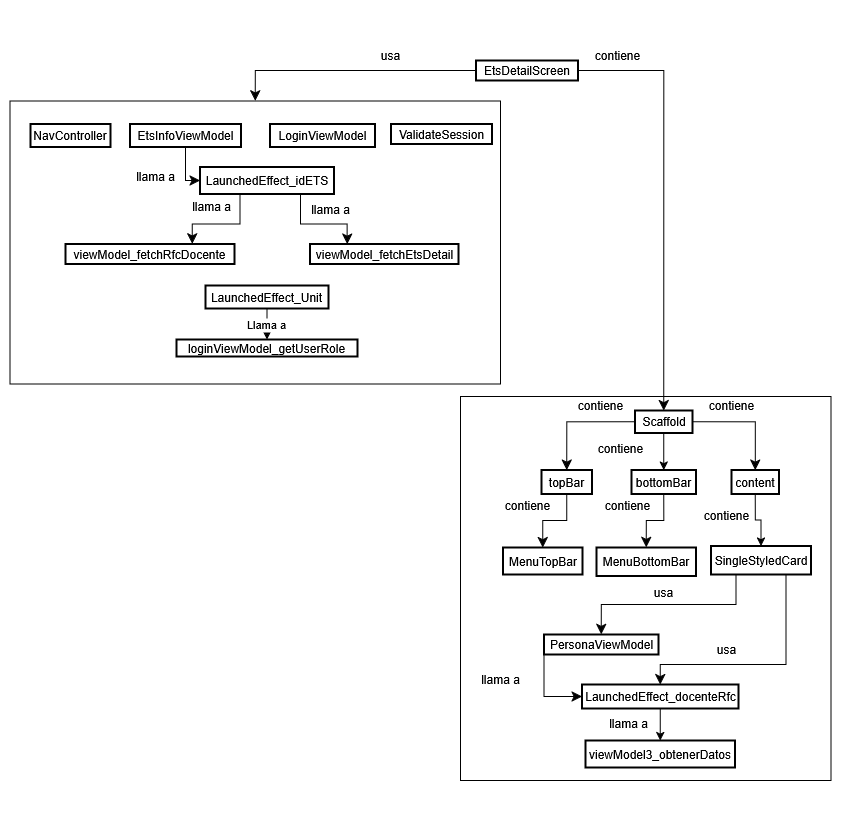
\includegraphics[width=0.9\textwidth]{DiagramasMoviles/DCM (20)}
		\caption{Diagrama de componentes para EtsDetailScreen.kt .}
		\label{fig:Componentes_7}
	\end{center}
\end{figure}

\newpage

\subsection{Diagrama de Componentes de EtsInscriptionProcessScreen.kt}

La Figura \ref{fig:Componentes_8} muestra el diagrama de componentes para ETSInscriptionProcessScreen.kt que es un composable que contiene a la \IUref{IU18}{Pantalla de Detalles del proceso de ETS}, que muestra la información necesaria para inscribirse a un ETS.

\begin{figure}[htbp!]
	\begin{center}
		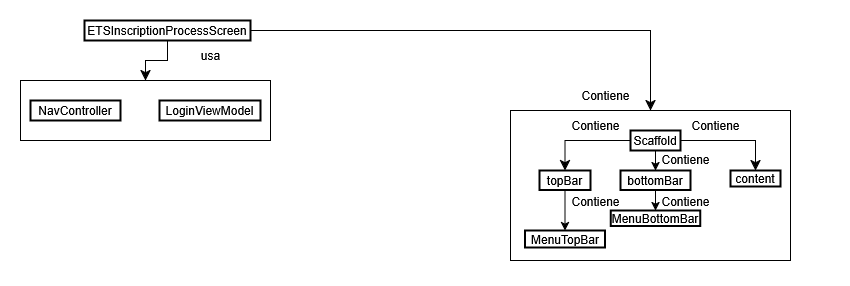
\includegraphics[width=0.9\textwidth]{DiagramasMoviles/DCM (21)}
		\caption{Diagrama de componentes para ETSInscriptionProcessScreen.kt .}
		\label{fig:Componentes_8}
	\end{center}
\end{figure}

\newpage

\subsection{Diagrama de Componentes de EtsListScreen.kt}

La Figura \ref{fig:Componentes_9} muestra el diagrama de componentes para EtsListScreen.kt que es un composable que contiene a la \IUref{IU05}{Pantalla Consultar ETS}, que muestra la lista de ETS del docente.

\begin{figure}[htbp!]
	\begin{center}
		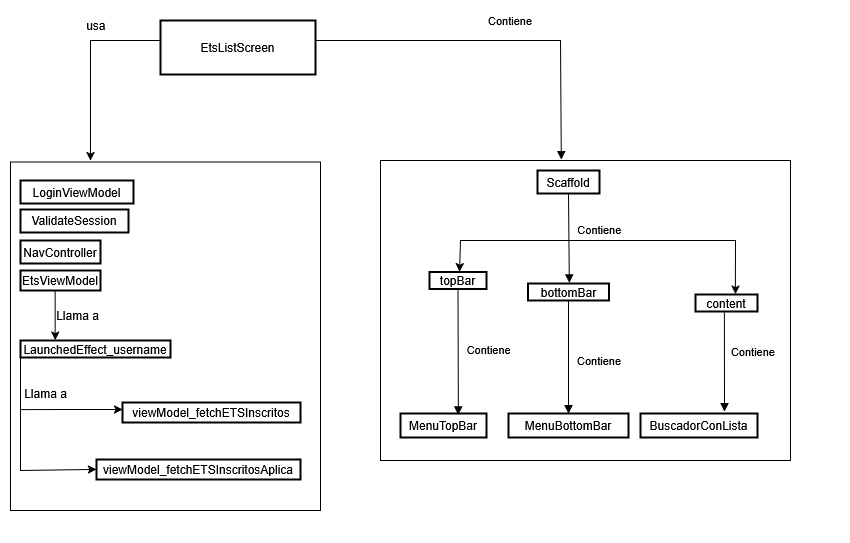
\includegraphics[width=0.9\textwidth]{DiagramasMoviles/DCM (22)}
		\caption{Diagrama de componentes para EtsListScreen.kt .}
		\label{fig:Componentes_9}
	\end{center}
\end{figure}

\newpage

\subsection{Diagrama de Componentes de EtsListScreenAlumno.kt}

La Figura \ref{fig:Componentes_10} muestra el diagrama de componentes para EtsListScreenAlumno.kt que es un composable que contiene a la \IUref{IU05}{Pantalla Consultar ETS}, que muestra la lista de ETS del alumno.

\begin{figure}[htbp!]
	\begin{center}
		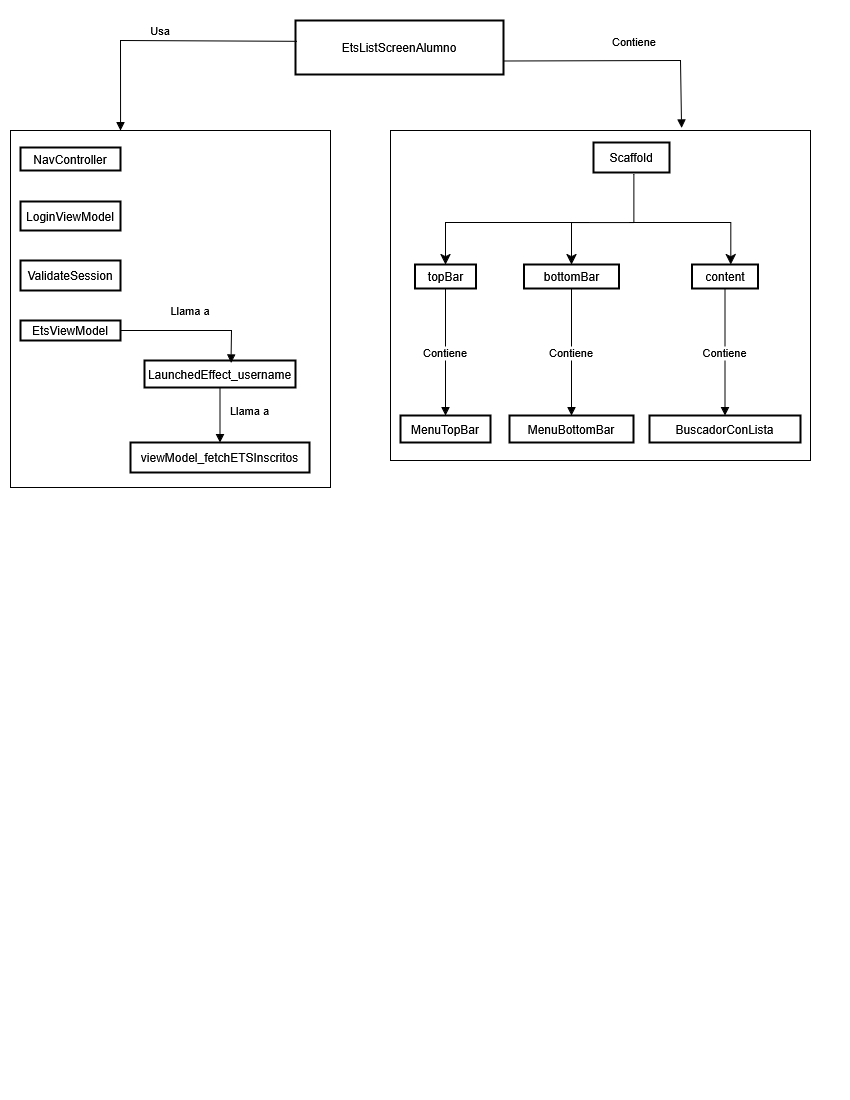
\includegraphics[width=0.9\textwidth]{DiagramasMoviles/DCM (23)}
		\caption{Diagrama de componentes para EtsListScreenAlumno.kt .}
		\label{fig:Componentes_10}
	\end{center}
\end{figure}

\newpage

\subsection{Diagrama de Componentes de InformacionAlumno.kt}

La Figura \ref{fig:Componentes_11} muestra el diagrama de componentes para InformacionAlumno.kt que es un composable que contiene a la \IUref{IUE07}{Creación del reporte}, que se utiliza para la creación de reportes y a su vez muestra la información esencial del alumno seleccionado.

\begin{figure}[htbp!]
	\begin{center}
		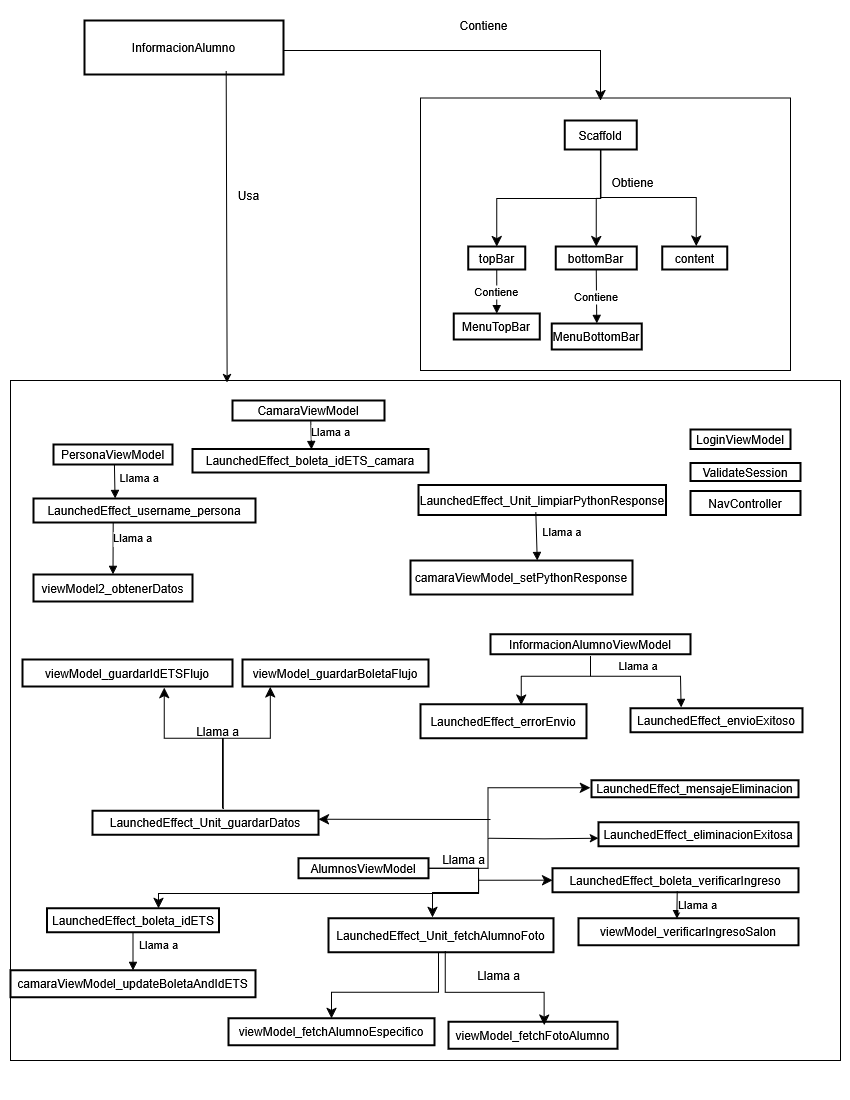
\includegraphics[width=0.7\textwidth]{DiagramasMoviles/DCM (24)}
		\caption{Diagrama de componentes para InformacionAlumno.kt .}
		\label{fig:Componentes_11}
	\end{center}
\end{figure}

\newpage

\subsection{Diagrama de Componentes de ListaAlumnosScreen.kt}

La Figura \ref{fig:Componentes_12} muestra el diagrama de componentes para ListaAlumnosScreen.kt que es un composable que contiene a la \IUref{IU08}{Pantalla Lista de asistencia de ETS}, que es la que le muestra la lista de alumnos inscritos a un ETS al docente, junto con su estado de asistencia con un icono.

\begin{figure}[htbp!]
	\begin{center}
		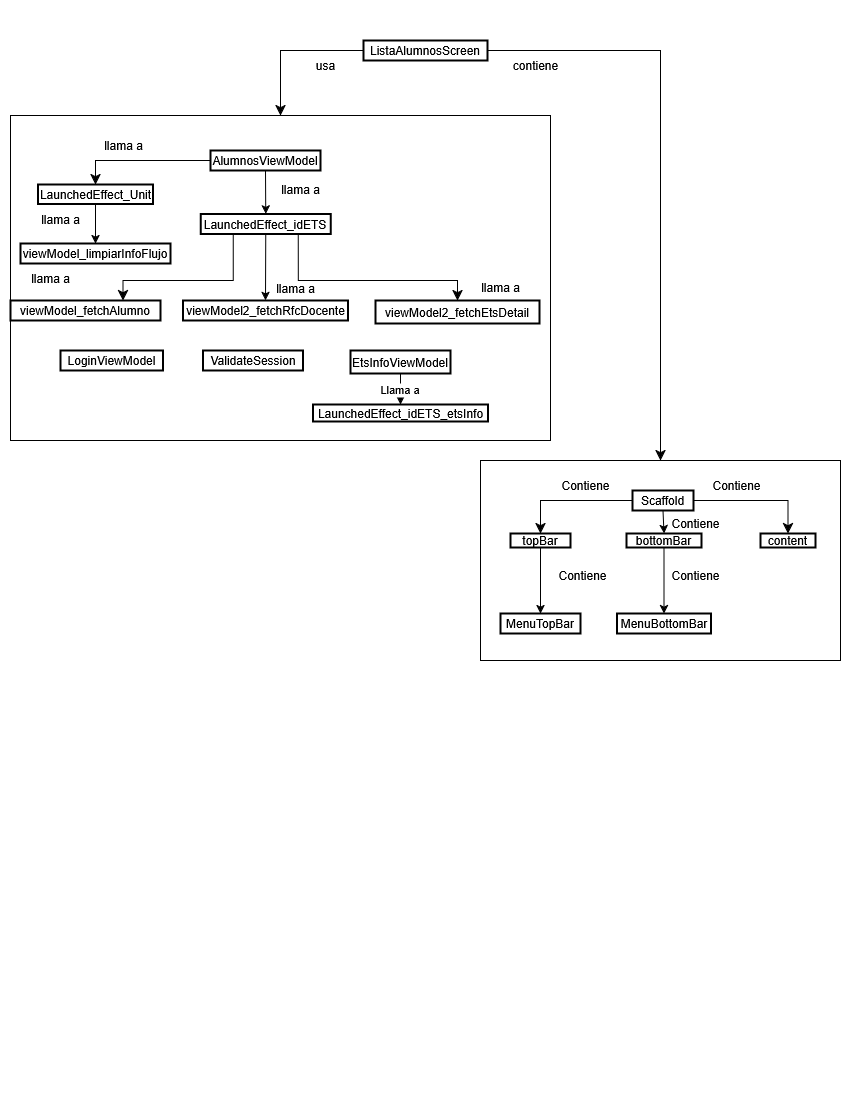
\includegraphics[width=0.9\textwidth]{DiagramasMoviles/DCM (25)}
		\caption{Diagrama de componentes para ListaAlumnosScreen.kt .}
		\label{fig:Componentes_12}
	\end{center}
\end{figure}

\newpage

\subsection{Diagrama de Componentes de ListadoSolicitudesReemplazo.kt}

La Figura \ref{fig:Componentes_13} muestra el diagrama de componentes para ListadoSolicitudesReemplazo.kt que es un composable que contiene una pantalla dedica a la visualización de las solicitudes de reemplazo y sus estados de aceptación o denegación. 

\begin{figure}[htbp!]
	\begin{center}
		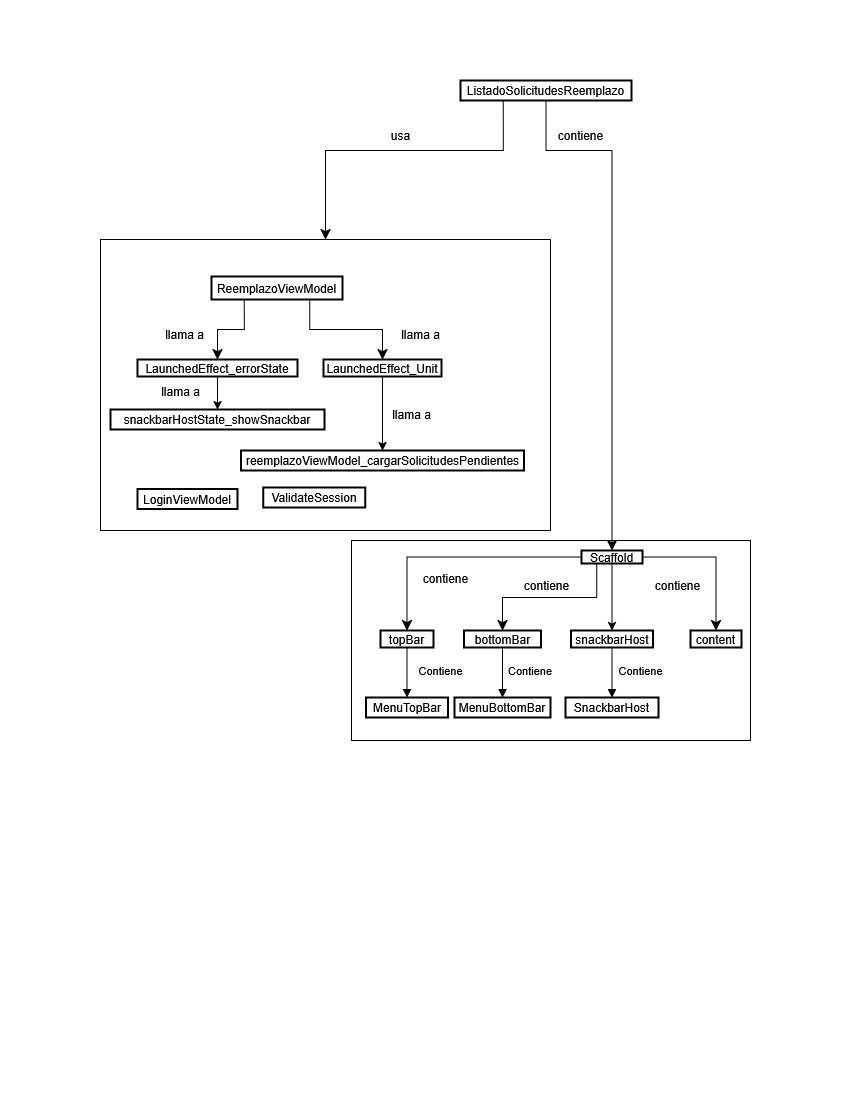
\includegraphics[width=0.9\textwidth]{DiagramasMoviles/DCM (26)}
		\caption{Diagrama de componentes para ListadoSolicitudesReemplazo.kt .}
		\label{fig:Componentes_13}
	\end{center}
\end{figure}

\newpage

\subsection{Diagrama de Componentes de LoginScreen.kt}

La Figura \ref{fig:Componentes_14} muestra el diagrama de componentes para LoginScreen.kt que es un composable que contiene a la \IUref{IU01}{Pantalla Iniciar sesión del sistema móvil}, que es el login de la aplicación móvil.

\begin{figure}[htbp!]
	\begin{center}
		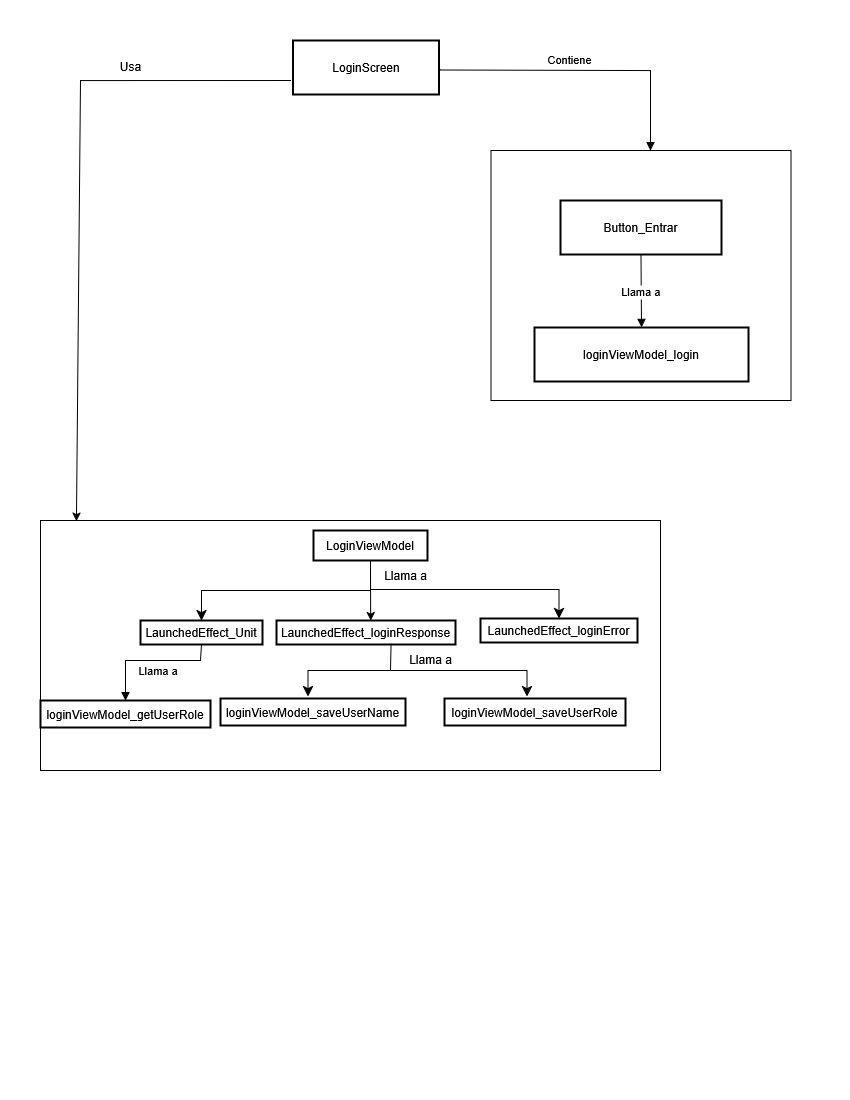
\includegraphics[width=0.9\textwidth]{DiagramasMoviles/DCM (27)}
		\caption{Diagrama de componentes para LoginScreen.kt .}
		\label{fig:Componentes_14}
	\end{center}
\end{figure}

\newpage

\subsection{Diagrama de Componentes de MensajesScreen.kt}

La Figura \ref{fig:Componentes_15} muestra el diagrama de componentes para MensajesScreen.kt que es un composable que es la pantalla donde se ven los mensaje específicos mandados a otro usuario.

\begin{figure}[htbp!]
	\begin{center}
		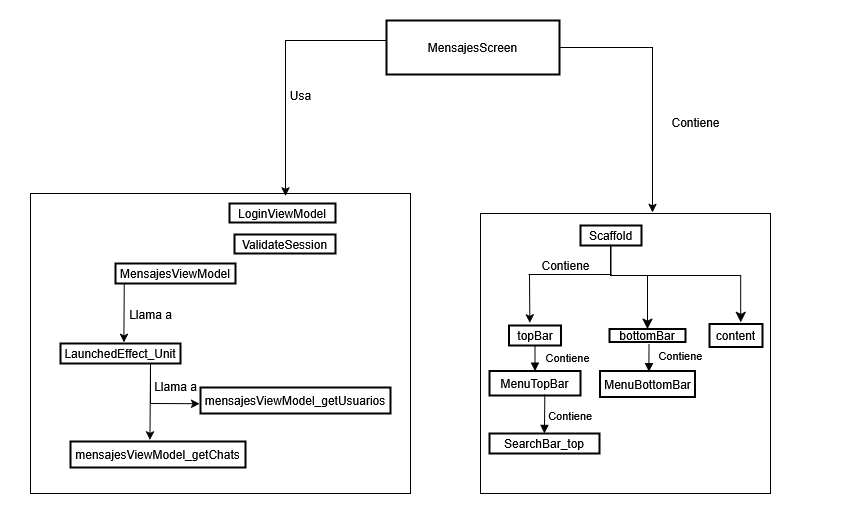
\includegraphics[width=0.9\textwidth]{DiagramasMoviles/DCM (28)}
		\caption{Diagrama de componentes para MensajesScreen.kt .}
		\label{fig:Componentes_15}
	\end{center}
\end{figure}

\newpage

\subsection{Diagrama de Componentes de QRScannerScreen.kt}

La Figura \ref{fig:Componentes_16} muestra el diagrama de componentes para QRScannerScreen.kt que es un composable que contiene a la \IUref{IU10}{Pantalla Código QR}, que muestra la cámara para poder escanear el código QR de la credencial del alumno.

\begin{figure}[htbp!]
	\begin{center}
		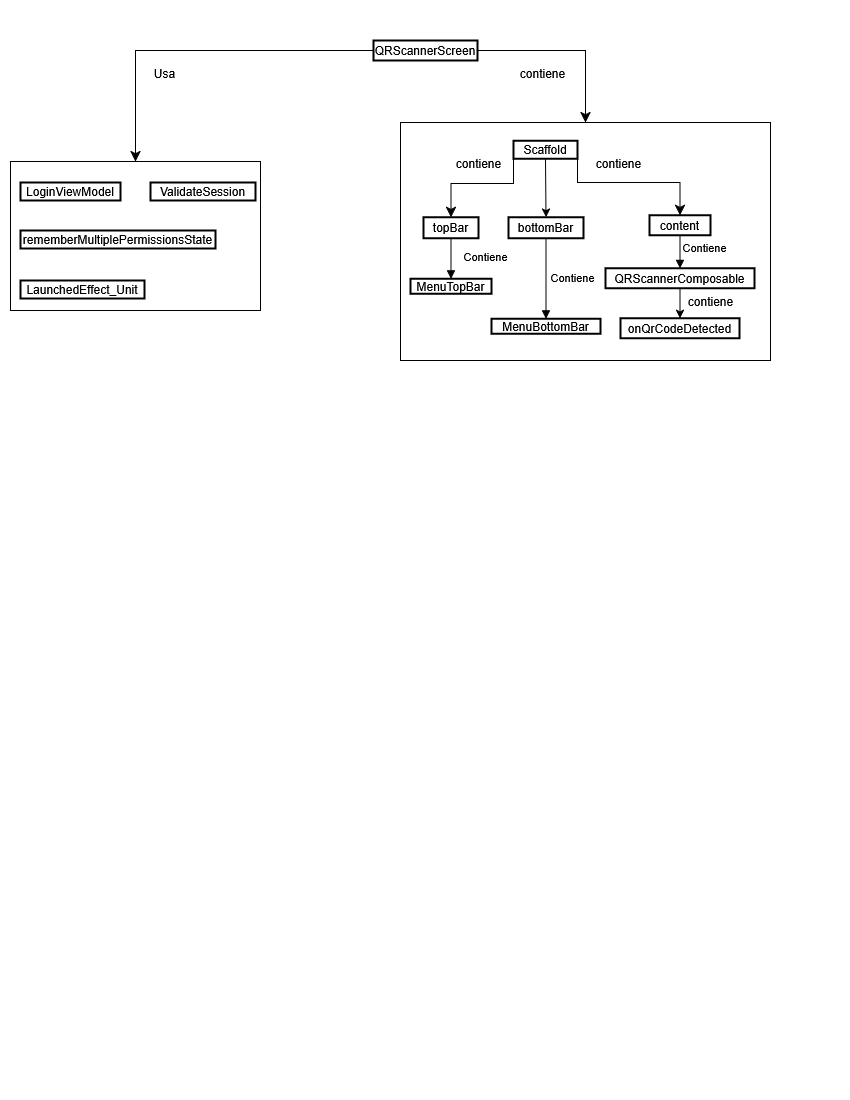
\includegraphics[width=0.9\textwidth]{DiagramasMoviles/DCM (29)}
		\caption{Diagrama de componentes para QRScannerScreen.kt .}
		\label{fig:Componentes_16}
	\end{center}
\end{figure}

\newpage

\subsection{Diagrama de Componentes de ReporteScreen.kt}

La Figura \ref{fig:Componentes_17} muestra el diagrama de componentes para ReporteScreen.kt que es un composable que contiene a la \IUref{IU20}{Pantalla Reporte del Alumno}, que es donde el docente puede revisar el reporte de la asistencia del alumno.

\begin{figure}[htbp!]
	\begin{center}
		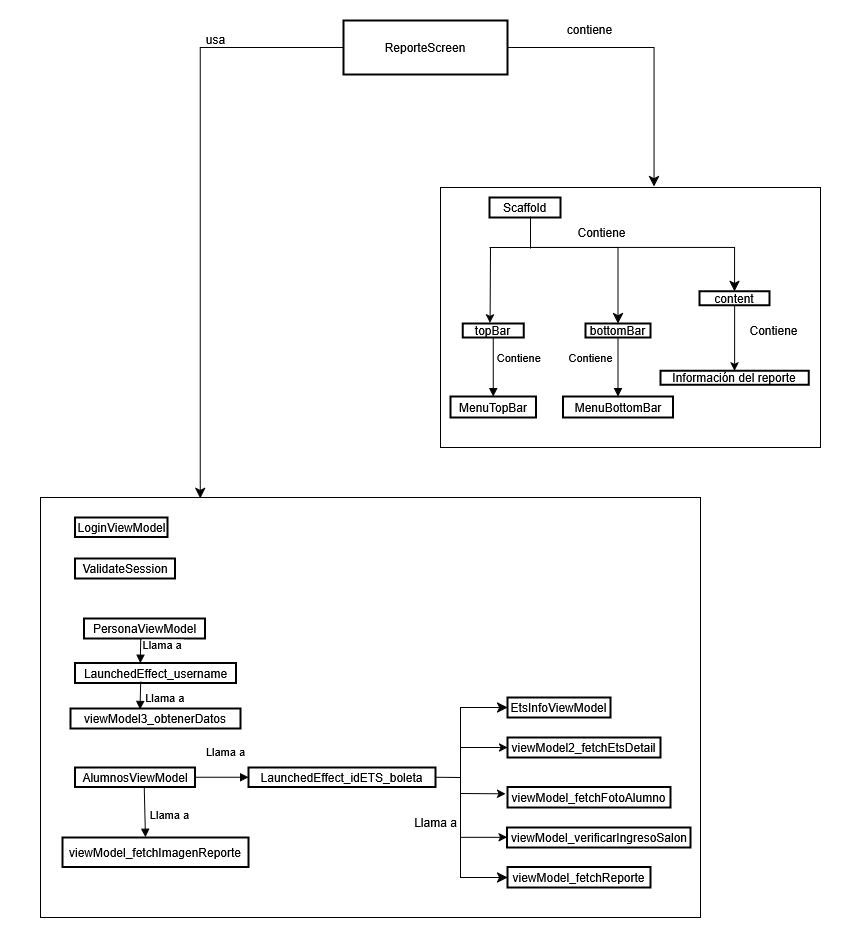
\includegraphics[width=0.7\textwidth]{DiagramasMoviles/DCM (30)}
		\caption{Diagrama de componentes para ReporteScreen.kt .}
		\label{fig:Componentes_17}
	\end{center}
\end{figure}

\newpage

\subsection{Diagrama de Componentes de ScreenAsignarremplazo.kt}

La Figura \ref{fig:Componentes_18} muestra el diagrama de componentes para ScreenAsignarremplazo.kt que es un composable que contiene a la pantalla \IUref{IU09}{Asignar docente de remplazo}, que es donde el jefe de departamento y/o el presidente de academia pueden responder a las solicitudes de reemplazo.

\begin{figure}[htbp!]
	\begin{center}
		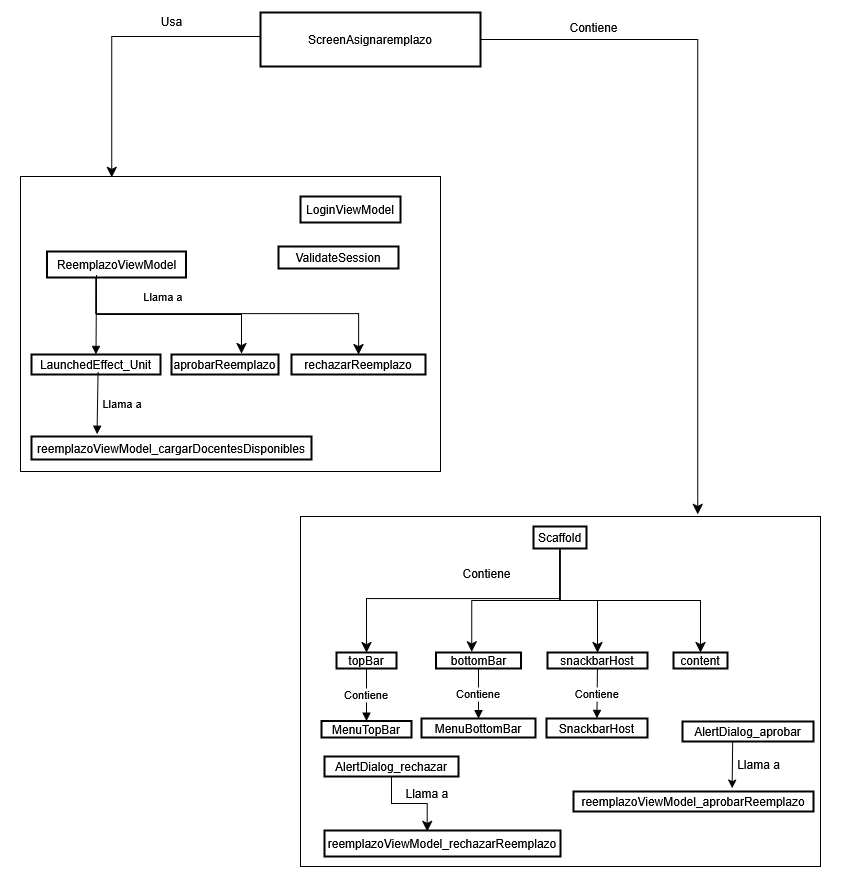
\includegraphics[width=0.9\textwidth]{DiagramasMoviles/DCM (31)}
		\caption{Diagrama de componentes para ScreenAsignarremplazo.kt .}
		\label{fig:Componentes_18}
	\end{center}
\end{figure}

\newpage

\subsection{Diagrama de Componentes de SolicitarReemplazo.kt}

La Figura \ref{fig:Componentes_19} muestra el diagrama de componentes para SolicitarReemplazo.kt que es un composable que contiene a la \IUref{IU07}{Pantalla de Solicitar remplazo}, que es donde el docente puede pedir un reemplazo como aplacador del ETS.

\begin{figure}[htbp!]
	\begin{center}
		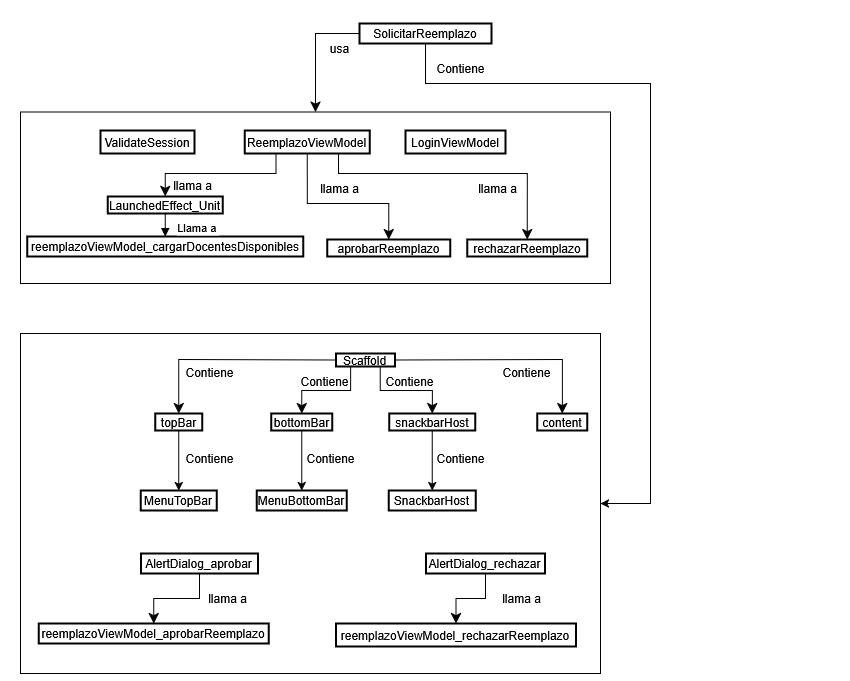
\includegraphics[width=0.9\textwidth]{DiagramasMoviles/DCM (32)}
		\caption{Diagrama de componentes para SolicitarReemplazo.kt .}
		\label{fig:Componentes_19}
	\end{center}
\end{figure}

\newpage

\subsection{Diagrama de Componentes de WelcomeScreen.kt}

La Figura \ref{fig:Componentes_20} muestra el diagrama de componentes para WelcomeScreen.kt que es un composable que contiene a la \IUref{IUE02}{Pantalla de saludo del personal de seguridad}, que es la pantalla de inicio del personal de seguridad (donde pude seleccionar la operación que quiere realizar y ver un saludo con su nombre).

\begin{figure}[htbp!]
	\begin{center}
		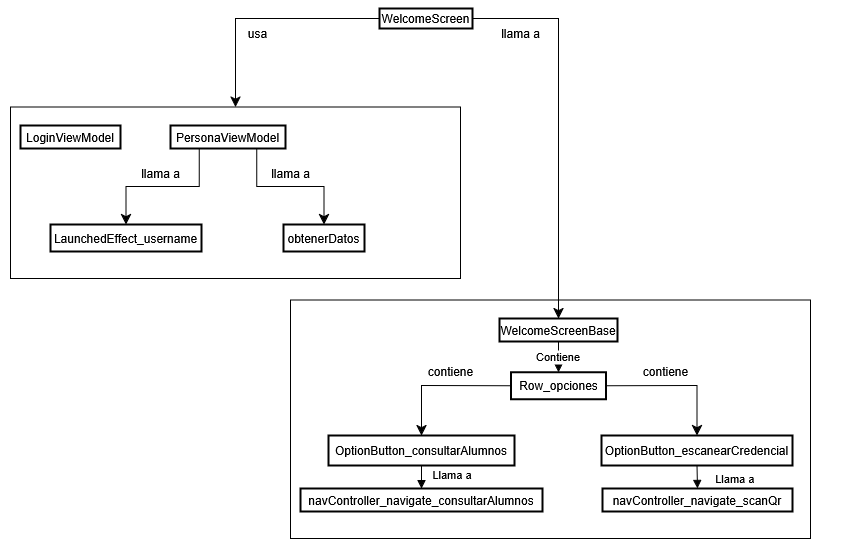
\includegraphics[width=0.9\textwidth]{DiagramasMoviles/DCM (33)}
		\caption{Diagrama de componentes para WelcomeScreen.kt .}
		\label{fig:Componentes_20}
	\end{center}
\end{figure}

\newpage

\subsection{Diagrama de Componentes de WelcomeScreenAcademico.kt}

La Figura \ref{fig:Componentes_21} muestra el diagrama de componentes para WelcomeScreenAcademico.kt que es un composable que contiene a la pantalla \IUref{IUE06}{saludo del presidente de academia y el jefe de departamento}, que es la pantalla de inicio del jefe de departamento y/o el presidente de academia (donde pude seleccionar la operación que quiere realizar y ver un saludo con su nombre).

\begin{figure}[htbp!]
	\begin{center}
		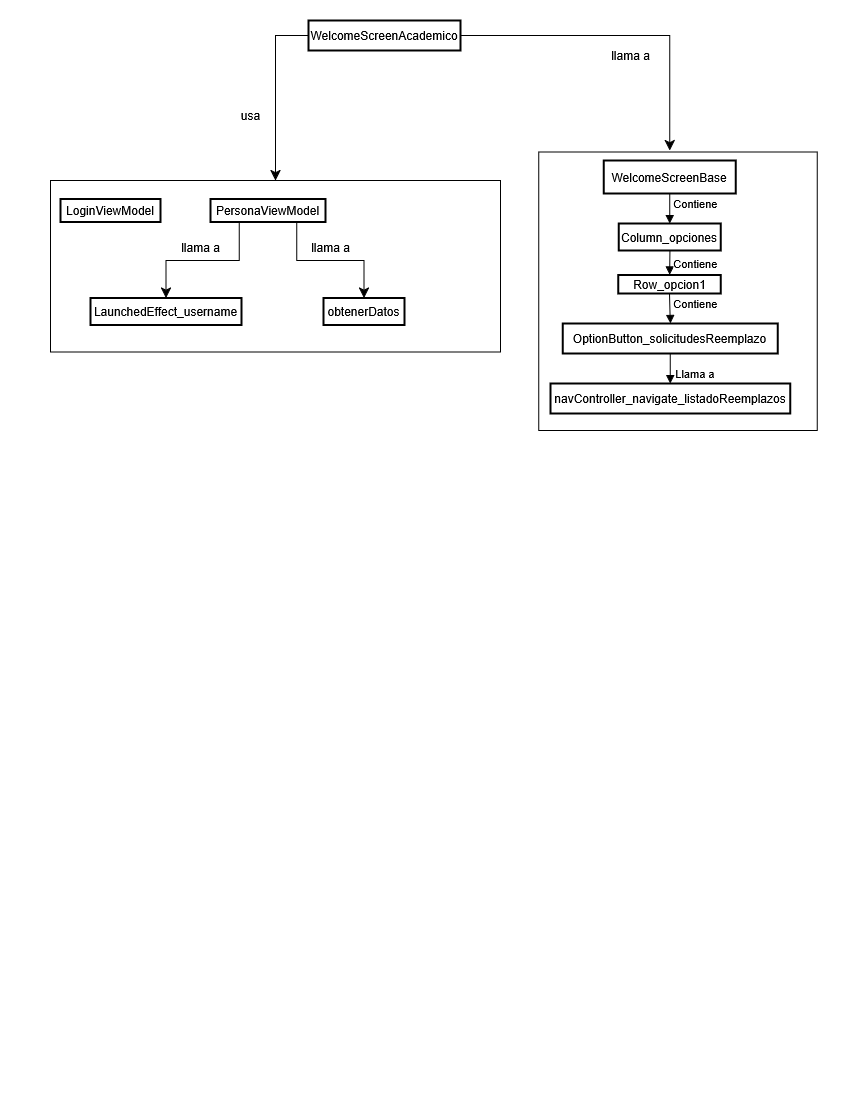
\includegraphics[width=0.9\textwidth]{DiagramasMoviles/DCM (34)}
		\caption{Diagrama de componentes para WelcomeScreenAcademico.kt .}
		\label{fig:Componentes_21}
	\end{center}
\end{figure}

\newpage

\subsection{Diagrama de Componentes de WelcomeScreenAlumno.kt}

La Figura \ref{fig:Componentes_22} muestra el diagrama de componentes para WelcomeScreenAlumno.kt que es un composable que contiene a la pantalla \IUref{IUE03}{Pantalla saludo del alumno}, que es la pantalla de inicio del Alumno (donde pude seleccionar la operación que quiere realizar y ver un saludo con su nombre).

\begin{figure}[htbp!]
	\begin{center}
		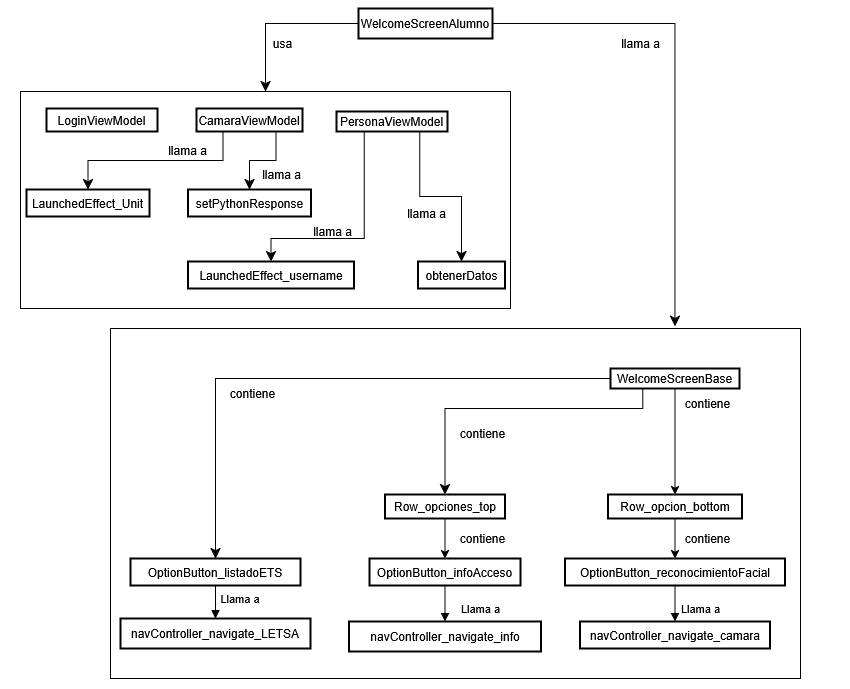
\includegraphics[width=0.9\textwidth]{DiagramasMoviles/DCM (35)}
		\caption{Diagrama de componentes para WelcomeScreenAlumno.kt .}
		\label{fig:Componentes_22}
	\end{center}
\end{figure}

\newpage

\subsection{Diagrama de Componentes de WelcomeScreenDocente.kt}

La Figura \ref{fig:Componentes_23} muestra el diagrama de componentes para WelcomeScreenDocente.kt que es un composable que contiene a la pantalla \IUref{IUE01}{Pantalla saludo de docente}, que es la pantalla de inicio del Docente (donde pude seleccionar la operación que quiere realizar y ver un saludo con su nombre).

\begin{figure}[htbp!]
	\begin{center}
		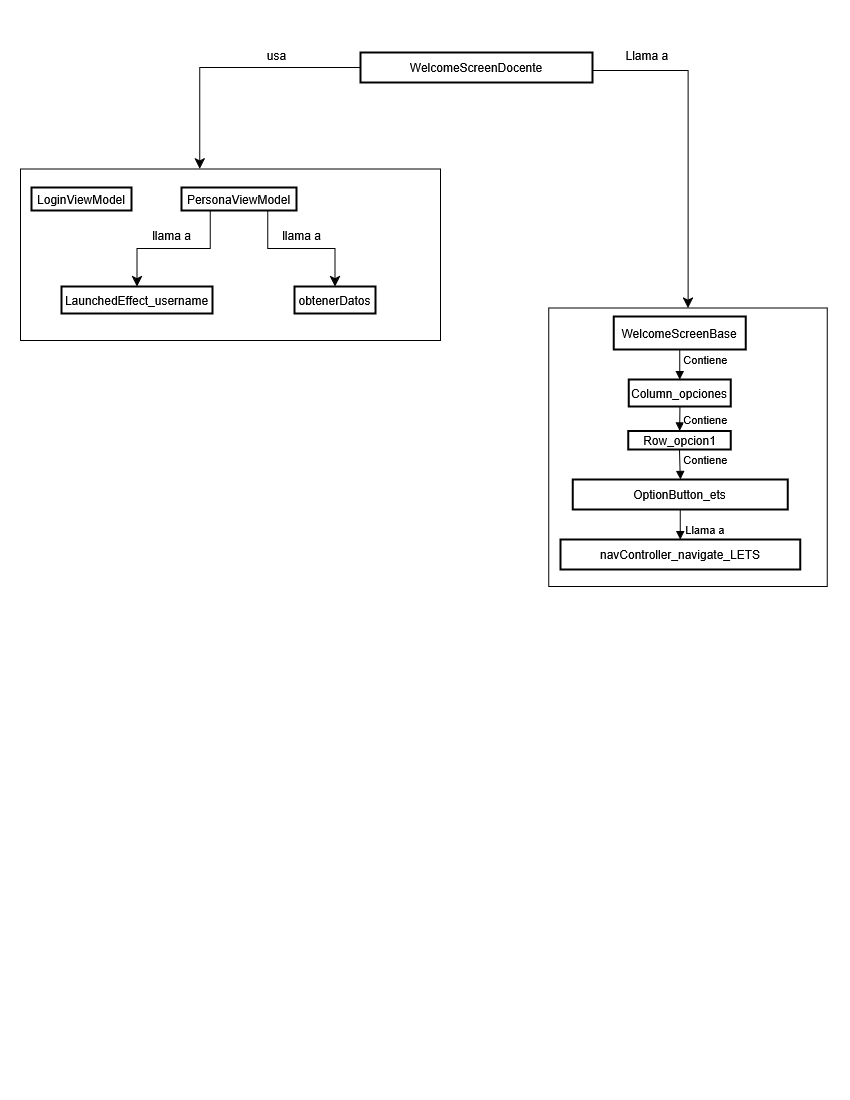
\includegraphics[width=0.8\textwidth]{DiagramasMoviles/DCM (36)}
		\caption{Diagrama de componentes para WelcomeScreenDocente.kt .}
		\label{fig:Componentes_23}
	\end{center}
\end{figure}